\chapter{Programmation mixte entière}
\label{chap:integer}

\section{Présentation générale}

Certaines quantités ne peuvent s'écrire sous forme de nombres réels, issus d'un domaine continu. Au contraire, certaines décisions sont par nature discrètes, et doivent se représenter à l'aide de nombres entiers.
Considérons par exemple une entreprise de transport, qui décide de renouvellement sa flotte de camions.
Le nombre de camions à acheter est un nombre naturel.

La présence de telles variables entières modifie profondément la nature des programmes sous-jacents.
Lorsqu'un problème est linéaire avec des variables entières, nous parlerons de {\sl programmation mixte entière}.
Si toutes les variables sont entières, nous utiliserons la terminologie de de {\sl programmation (pure) en nombres entiers}.
Un exemple de programme en nombres entiers a déjà été rencontré dans la Sectionn~\ref{sec:ex_villes}.
Si les variables entières sont à valeurs 0 ou 1 (binaires), nous parlerons de programmatión 0--1 (binaire).

Nous pourrions bien entendu considérer le cas non-linéaire, mais les complications sont telles qu'à ce jour, aucune méthode pleinement satisfaisante n'existe, même si d'intenses recherches sont actuellement conduites à ce niveau, notamment au sein de l'entreprise IBM.

\begin{example}[Problème du sac à dos]
Considérons un cambrioleur muni d'un sac (unique) pour transporter son butin.
Son problème consiste à maximiser la valeur totale des objets qu'il emporte, sans toutefois dépasser une limite de poids $b$ correspondant à ses capacités physiques.
Supposons qu'il y a $n$ type d'objets que le voleur pourrait emporter, et que ceux-ci sont en nombre tel que quelle que soit la nature de l'objet considéré, la seule limite au nombre d'unités que le cambrioleur peut prendre est que le poids total reste inférieur à $b$.
Si l'on associe à l'objet $j$ une valeur $c_j$ et un poids $w_j$, la combinaison optimale
d'objets à emporter sera obtenue en résolvant le programme mathématique
\begin{align*}
\max_x\ & \sum_{j = 1}^n c_j x_j \\
\text{s.c. } & \sum_{j = 1}^n w_j x_j \leq b \\
& x_j \in \NN, \ j = 1,\ldots,n.
\end{align*}
Ici, $x_j \in \NN$ signifie que $x_j$ est un naturel, autrement dit un entier non négatif.
Intuitivement, nous pourrions penser que la solution consiste à choisir en premier lieu les objets dont le rapport qualité-poids est le plus avantageux, quitte à tronquer pour obtenir une solution entière (nous ne pouvons pas diviser un objet).
Cette solution peut malheureusement se révéler sous-optimale, voire mauvaise, comme on le constate sur l'exemple suivant.
\begin{align*}
\max_x \ & 2x_1 + 3x_2 + 7x_3 \\
\text{s.c. } & 3x_1 + 4x_2 + 8x_3 \leq 14,\\
& x_1,\ x_2,\ x_3 \in \NN.
\end{align*}
Si nous oublions la contrainte d'intégralité, la solution, de valeur $12.25$, est $x = (0, 0, 14/8)$.
En tronquant, on obtient la solution entière $x = (0, 0, 1)$ de valeur 7.
Il est facile de trouver de meilleures solutions, par exemple $x = (1, 0, 1)$.

La solution optimale du problème du cambrioleur peut s'obtenir en énumérant toutes les solutions admissibles et en conservant la meilleure (voir Table~\ref{tab:bagpack},
, où les solutions inefficaces laissant la possibilité d'ajouter un objet n'ont pas été considérées).

\begin{table}[htb]
\begin{center}
\begin{tabular}{cccc}
$x_1$ & $x_2$ & $x_3$ & objectif \\
\hline
0 & 1 & 1 & 10 \\
2 & 0 & 1 & 11 \\
0 & 3 & 0 & 9 \\
2 & 2 & 0 & 10 \\
3 & 1 & 0 & 9 \\
4 & 0 & 0 & 8 \\
\hline
\end{tabular}
\caption{Problème du sac à dos: énumération des solutions}
\label{tab:bagpack}
\end{center}
\end{table}

La solution optimale entière, $x = (2, 0, 1)$, diffère passablement de la solution optimale linéaire.
Cependant, il est clair que cette technique d'énumération ne peut s'appliquer à des problèmes de grande taille.
\end{example}

\begin{example}[California Mfg]
Une entreprise doir choisir de nouveaux emplacements pour construire des usines et
des entrepôts.
Elle a le choix entre deux emplacements: Los Angeles (LA) et San Fransisco (SF).
Nous ne pouvons construire un entrepôt que dans une ville où nous disposons d'une usine, et nous ne pouvons pas construire plus d'un entrepôt.
Nous associons à chaque construction (d'une usine ou d'un entrepôt dans chacun des lieux envisagés) sa valeur estimée et son coût de construction.
L'objectif est de maximiser la valeur totale estimée, en ne dépassant pas une limite maximum sur les coûts.
Les données du problème sont résumées dans la Table~\ref{tab:california}.
\begin{table}
\begin{center}
\begin{tabular}{|l|c|c|}
\hline
& Valeur estimée (millions \$) & Coût de construction (millions \$) \\
\hline
Usine à LA & 9 & 6 \\
\hline
Usine à SF & 5 & 3 \\
\hline
Entrepôt à LA & 6 & 5 \\
\hline
Entrepôt à SF & 4 & 2 \\
\hline
Limite maximum & - & 10 \\
\hline
\end{tabular}
\caption{Données du problème California Mfg}
\label{tab:california}
\end{center}
\end{table}
Les variables sont
\[
x_j =
\begin{cases}
1 & \mbox{ si la décision $j$ est approuvée;} \\
0 & \mbox{ si la décision $j$ n'est pas approuvée.}
\end{cases}
\]
L'objectif est de maximiser la valeur estimée totale:
\[
\max z = 9x_1 + 5x_2 + 6x_3 + 4x_4.
\]
Les contraintes fonctionnelles sont
\begin{enumerate}
\item
la limite maximum sur les coûts de construction:
\[
6x_1 + 3x_2 + 5x_3 + 2x_4 \leq 10;
\]
\item
nous ne pouvons construire plus d'un entrepôt:
\[
x_3 + x_4 \leq 1;
\]
\item
l'entrepôt ne sera à LA que si l'usine est à LA:
\[
x_3 \leq x_1;
\]
\item
l'entrepôt ne sera à SF que si l'usine est à SF:
\[
x_4 \leq x_2:
\]
\item
contraintes 0--1 (intégralité):
\[
x_j \in \lbrace 0, 1 \rbrace,\ j = 1, 2, 3, 4;
\]
ou encore
\[
0 \leq x_j \leq 1 \mbox{ et } x_j \mbox{ entier},\ j = 1, 2, 3, 4.
\]
\end{enumerate}
Par conséquent, nous avons le programme mathématique
\begin{align*}
max\ & z = 9x_1 + 5x_2 + 6x_3 + 4x_4 \\
\st & 6x_1 + 3x_2 + 5x_3 + 2x_4 \leq 10; \\
& x_3 + x_4 \leq 1; \\
& -x_1 + x_3 \leq 0; \\
& -x_2 + x_4 \leq 0; \\
& x_1, x_2, x_3, x_4 \leq 1; \\
& x_1, x_2, x_3, x_4 \geq 0; \\
& x_1, x_2, x_3, x_4 \mbox{ entiers}.
\end{align*}
Le modèle illustre deux cas classiques d'illustrations de variables binaires:
\begin{itemize}
\item
alternatives mutuellement exclusives: nous ne pouvons construire plus d'un entrepôt, i.e.
\[
x_3 + x_4 \leq 1;
\]
\item
décisions contingentes: nous ne pouvons construire un entrepôt que là où nous avons construit une usine:
\begin{align*}
x_3 \leq x_1;
x_4 \leq x_2:
\end{align*}
\end{itemize}
\end{example}

\begin{example}[Localisation]
Une entreprise envisage plusieurs sites de construction pour des usines qui serviront à approvisionner ses clients.
\`A chaque site potentiel $i$ correspond un coût de construction $a_i$, une capacité de production $u_i$, un coût de production unitaire $b_i$ et des coûts de transport $c_{ij}$ des usines vers les clients.
Soit $y_i$ une variable binaire prenant la valeur 1 si un entrepôt est construit sur le site $i$, $d_j$ la demande de l'usine $j$ et $x_{ij}$ la quantité produite à l'usine $i$ et destinée au marché $j$ (flot de $i$ à $j$).
Un plan de construction optimal est obtenu en résolvant le programme
\begin{align*}
\min_x\ & \sum_i a_iy_i + \sum_i b_i \sum_j x_{ij} + \sum_i \sum_j c_{ij}x_{ij} \\
\text{s.c. } & \sum_i x_{ij} = d_j, \\
& \sum_j x_{ij} \leq u_iy_i, \\
& x_{ij} \geq 0, \\
& y_i \in \lbrace 0, 1 \rbrace.
\end{align*}
Cette formulation contient deux éléments intéressants: un coût fixe (construction) modélisé par une variable binaire $y_i$ ainsi qu'une contrainte logique forçant les flots provenant d'un site à être nuls si aucune usine n'est construite en ce site.
Notons aussi que certaines variables sont entières alors que d'autres (flots) sont
réelles.
\end{example}

\begin{example}[Contraintes logiques]
Des variables binaires peuvent servir à représenter des contraintes logiques.
En voici quelques exemples, où $p_i$ représente une proposition logique et $x_i$ la variable logique (binaire) correspondante.
\begin{center}
\begin{minipage}{0.4\textwidth}
contrainte logique\\
$p_1 \oplus p_2 =$ vrai \\
$p_1 \lor p_2 \lor \dots \lor p_n =$ vrai \\
$p_1 \land p_2 \land \ldots \land p_n =$ vrai \\
$p_1 \Rightarrow p_2$ \\
$p_1 \Leftrightarrow p_2$
\end{minipage}
\begin{minipage}{0.4\textwidth}
 forme algébrique \\
$x1 + x2 = 1$ \\
$x_1 + x_2 + \ldots + x_n \geq 1$ \\
$x_1 + x_2 + \ldots + x_n \geq n$ (ou $= n$) \\
$x_2 \geq x_1$ \\
$x_2 = x_1$
\end{minipage}
\end{center}
\end{example}

\begin{example}[Fonctions linéaires par morceaux]
Considérons une fonction objectif à maximiser, pour laquelle dans chaque intervalle
$[a_{i-1}, a_i]$ la fonction est linéaire, ce que nous pouvons exprimer par:
\begin{align*}
& x = \lambda_{i-1}a_{i-1} + \lambda_ia_i \\
& \lambda_{i-1} + \lambda_i = 1, \\
& \lambda_{i-1},\ \lambda_i \geq 0, \\
& f(x) = \lambda_{i-1}f(a_{i-1}) + \lambda_if(a_i).
\end{align*}
Nous pouvons généraliser cette formule sur tout l'intervalle de définition de la fonction $f$ en contraignant les variables $\lambda_i$ à ne prendre que deux valeurs non nulles, et ce pour deux indices consécutifs.
Ceci se fait en introduisant des variables binaires $y_i$ associées aux intervalles de linéarité $[a_{i-1}, a_i]$:
\begin{align*}
x &= \sum_{i = 0}^n \lambda_i a_i, \\
f(x) &= \sum_{i = 0}^n \lambda_i f(a_i), \\
\sum_{i = 0}^n \lambda_i &= 1, \\
\lambda_i & \geq 0,\ i = 0,\ldots, n \\
\lambda_0 & \leq y_1, \\
\lambda_1 & \leq y1 + y2, \\
\vdots\ &\ \vdots\qquad \vdots \\
\lambda_{n-1} & \leq y_{n-1} + y_n, \\
\lambda_n & \leq y_n,\\
\sum_{i = 1}^n y_i & = 1 \mbox{(un seul intervalle ``actif'')} \\
y_i & \in {0, 1},\ i = 1,\ldots, n.
\end{align*}

Si la fonction $f$ est concave, les variables binaires $y_i$ et les contraintes associées peuvent être éliminées de la formulation.
Cette approche est particulièrement intéressante lorsqu'on optimise des fonctions de plusieurs variables de la forme $\sum_i f_i(x_i)$.
\end{example}

\section{Contraintes mutuellement exclusives}

\subsection{Deux contraintes}

Prenons l'exemple de deux contraintes.
L'une ou l'autre des deux contraintes doit être satisfaite, mais pas les deux simultanément. Par exemple,
\begin{itemize}
\item
soit $3x_1 + 2x_2 \leq 18$;
\item
soit $x_1 + 4x_2 \leq 16$.
\end{itemize}
Soit $M$ un très grand nombre; le système précédent est équivalent à
\begin{itemize}
\item
soit
\begin{align*}
3x_1 + 2x_2 \leq 18,\\
x_1 + 4x_2 \leq 16 + M;
\end{align*}
\item
soit
\begin{align*}
3x_1 + 2x_2 & \leq 18 + M,\\
x_1 + 4x_2 & \leq 16.
\end{align*}
\end{itemize}
En introduisant une variable binaire $y$, nous obtenons le système équivalent
\begin{align*}
3x_1 + 2x_2 &\leq 18 + M(1-y), \\
x_1 + 4x_2 &\leq 16 +My.
\end{align*}
La signification de cette variable est
\begin{itemize}
\item
$y = 1$, si la première contrainte est satisfaite;
\item
$y = 0$, si la seconde contrainte est satisfaite.
\end{itemize}
Nous avons de la sorte construit deux alternatives mutuellement exclusives.

Nous aurions pu aussi introduire deux variables binaires:
\begin{itemize}
\item
$y_1 = 1$, si la première contrainte est satisfaite;
\item
$y_2 = 1$, si la seconde contrainte est satisfaite.
\end{itemize}
Nous devons avoir
\[
y_1 + y_2 = 1.
\]
Afin de se ramener au modèle précédent, il suffit de poser
\begin{align*}
y_1 &= y; \\
y_2 &= 1-y.
\end{align*}
Il s'agit d'un cas particulier de la situation suivante: $K$ parmi $N$ contraintes doivent être satisfaites.
Dans ce cas plus général, nous introduisons $N$ variables binaires.

\subsection{$K$ contraintes parmi $N$}

Soit les $N$ contraintes
\[
f_j(x_1,x_2,\ldots,x_n) \leq d_j,\ j = 1,2,\ldots,N.
\]
Nous introduisons $N$ variables binaires, avec $y_j = 1$ si la $j^e$ contrainte est satisfaite:
\[
f_j(x_1,x_2,\ldots,x_n) \leq d_j + M(1-y_j),\ j = 1,2,\ldots,N.
\]
Il reste à spécifier que seulement $K$ de ces contraintes peuvent êtres satisfaites:
\[
\sum_{j = 1}^N y_j = K.
\]

\subsection{Fonction ayant $N$ valeurs possibles}

Soit la contrainte
\[
f(x_1,x_2,\ldots,x_n) = d_1,\mbox{ ou }d_2\mbox{ ou }\ldots\mbox{ ou }d_N.
\]
Nous introduisons $N$ variables binaires, avec $y_j = 1$ si la fonction vaut $d_j$.
La contrainte s'écrit alors
\[
f(x_1,x_2,\ldots,x_n) = \sum_{j=1}^N d_j y_j,
\]
avec
\[
\sum_{j = 1}^N y_j = 1.
\]

\begin{example}[Wyndor Glass]
Supposons que le temps de production maximum à l'usine 3 n'est pas toujours 18h, mais pourrait également être 6h ou 12h.
Cette contrainte s'écrit alors
\[
3x_1 + 2x_2 = 6\mbox{ ou }12\mbox{ ou }18.
\]
Nous introduisons alors trois variables binaires
\begin{align*}
3x_1 + 2x_2 &= 6y_1 + 12y_2 + 18y_3,\\
y_1 + y_2 + y_3 &= 1.
\end{align*}
\end{example}

\subsection{Objectif avec coûts fixes}

Supposons que le coût associé à un produit $j$ est composé de deux parties:
\begin{enumerate}
\item
un coût fixe initial $k_j$ encouru dès qu'une unité de $j$ est produite;
\item
un coût $c_j$ proportionnel au nombre d'unités de $j$ produites.
\end{enumerate}
Le coût total associé à la production de $x_j$ unités est
\[
f(x_j) =
\begin{cases}
k_j + c_j x_j & \mbox{ si } x_j > 0,\\
0 & \mbox{ si } x_j = 0.
\end{cases}
\]

Supposons de plus que l'objectif consiste à minimiser la somme de $n$ fonctions avec coûts fixes
\[
\min z = \sum_{j=1}^n f_j(x_j).
\]
Nous introduisons alors $n$ variables binaires:
\[
y_j =
\begin{cases}
1 \mbox{ si } x_j > 0,\\
0 \mbox{ si } x_j = 0.
\end{cases}
\]
L'objectif s'écrit alors
\[
\min z = \sum_{j = 1}^n c_jx_j + k_jy_j.
\]
Les valeurs de $x_j$ et de $y_j$ dépendent l'une de l'autre: il s'agit d'un exemple de {\sl décisions contingentes}.
Nous devons en particulier avoir une contrainte qui précise que $x_j = 0$ si $y_j = 0$.
Toutefois, les deux variables ne sont plus binaires, vu que $x_j$ peut être quelconque.
Soit $M_j$ une borne supérieure sur la valeur de $x_j$.
Nous pouvons écrire la relation entre les deux variables de cette manière:
\[
x_j \leq M_jy_j.
\]
Ainsi,
\begin{itemize}
\item
si $y_j = 0$, alors $x_j = 0$;
\item
si $y_j = 1$, alors $x_j \leq M_j$;
\item
si $x_j > 0$, alors $y_j = 1$;
\item
si $x_j = 0$, alors toute soluton optimale satisfait $y_j = 0$ lorsque $k_j > 0$ (si $k_j = 0$, la variable $y_j$ est inutile).
\end{itemize}
Nous obtenons par conséquent le programme
\begin{align*}
\min\ & z = \sum_{j = 1}^n c_jx_j + k_jy_j\\
\st & x_j \leq M_j, \\
& y_j \in \lbrace 0,1 \rbrace,\ j = 1,2,\ldots,n.
\end{align*}

\subsection{Variables entières en variables 0--1}

Soit $x$ une variable entière générale bornée:
\[
0 \leq x \leq u,
\]
et soit $N$ l'entier tel que $2^N \leq u \leq 2^{N+1}$.
La représentation binaire de $x$ est
\[
x = \sum_{j = 0}^N 2^j y_j.
\]
L'intérêt de cette transformation est que les méthodes de programmation 0--1 sont souvent plus efficaces que les méthodes de programmation en nombres entiers.
Elle engendre néanmoins une multiplication du nombre de variables.

\begin{example}
Nous considérons trois types de produits, et deux usines; nous exprimons le profit par unité de produit en milliers de dollars.
Nous connaissons les ventes potentielles par produit (unités/semaine), et la capacité de production par usine (h/semaine).
Nous avons toutefois comme contrainte que pas plus de deux produits ne peuvent être fabriqués, et une seule des deux usines doit être exploitée.
Les données du problème sont résumées dans la Table~\ref{tab:prod_integer}.
\begin{table}[htb]
\begin{center}
\begin{tabular}{|l|c|c|c|c|}
\hline
& Produit 1 & Produit 2 & Produit 3 & Capacité de \\
& temps de production & temps de production & temps de production & production \\
& (h/unité) &(h/unité) &(h/unité) & (h/semaine) \\
\hline
Usine 1 & 3 & 4 & 2 & 30 \\
\hline
Usine 1 & 4 & 6 & 2 & 40 \\
\hline
Profit/unité& 5 & 7 & 3 & --\\
(1000\$) & & & & \\
\hline
Ventes potentielles & 7 & 5 & 9 & --\\
 (par semaine) & & & & \\
 \hline
\end{tabular}
\caption{Exemple de production avec variables entières.}
\label{tab:prod_integer}
\end{center}
\end{table}
Les variables sont $x_j$, le nombre d'unités fabriquées du produit $j$.
Pour représenter la contrainte ``pas plus de deux produits'', nous devons introduire des variables 0--1:
\[
y_j =
\begin{cases}
1 & \si x_j > 0; \\
0 & \si x_j = 0.
\end{cases}
\]
Afin de représenter la contrainte ``une seule des deux usines'', nous devons ajouter une variables 0--1:
\[
y_4 =
\begin{cases}
1 & \si \mbox{l'usine 1 est choisie}; \\
0 & \si \mbox{sinon}.
\end{cases}
\]
L'objectif est
\[
\max z = 5x_1 + 7x_2 + 3x_3.
\]
Les ventes potentielles sont
\[
x_1 \leq 7,\ x_2 \leq 5,\ x_3 \leq 9.
\]
L'exigence interdisant d'avoir plus de deux produits se traduit mathématiquement par
\[
y_1 + y_2 + y_3 \leq 2.
\]
La relation entre les variables continues et les variables 0--1 s'exprime par
\[
x_1 \leq 7y_1,\ x_2 \leq 5y_2,\ x_3 \leq 9y_3.
\]
La contrainte portant sur l'utilisation d'une seule usine est
\begin{itemize}
\item
soit $3x_1 + 4x_2 + 2x_3 \leq 30$;
\item
soit $4x_1 + 6x_2 + 2x_3 \leq 40$.
\end{itemize}
En utilisant la variable 0--1 (et $M$ très grand), elle se traduit par
\begin{align*}
3x_1 + 4x_2 + 2x_3 &\leq 30 + M(1-y_4), \\
4x_1 + 6x_2 + 2x_3 &\leq 40 + My_4.
\end{align*}
En résumé, nous avons le modèle
\begin{align*}
\max z &= 5x_1 + 7x_2 + 3x_3\\
\st & x_1 \leq 7y_1,\ x_2 \leq 5y_2,\ x_3 \leq 9y_3\\
& y_1 + y_2 + y_3 \leq 2,\\
& 3x_1 + 4x_2 + 2x_3 \leq 30 + M(1-y_4), \\
& 4x_1 + 6x_2 + 2x_3 \leq 40 + My_4, \\
& x_1, x_2, x_3 \geq 0,\\
& y_j \in \lbrace 0,1 \rbrace, j = 1,2,3,4.
\end{align*}
\end{example}

\begin{example}
Nous considérons à nouveau trois types de produits, pour lesquels nous pouvons placer cinq annonces publicitaires, avec un maximum de trois annonces par produit.
L'estimation des revenus publicitaires est donnée dans la Table~\ref{tab:ads}, où les profits sont exprimés en millions de dollars.
\begin{table}[htb]
\begin{center}
\begin{tabular}{|c|c|c|c|}
\hline
Nombre d'annonces & Produit 1 & Produit 2 & Produit 3 \\
\hline
0 & 0 & 0 & 0 \\
\hline
1 & 1 & 0 & -1 \\
\hline
2 & 3 & 2 & 2 \\
\hline
3 & 3 & 3 & 4 \\
\hline
\end{tabular}
\caption{Revenus publicitaires.}
\label{tab:ads}
\end{center}
\end{table}
Les variables du problèmes sont le nombre d'annonces pour le produit $i$, dénoté par $x_i$, mais l'hypothèse de proportionnalité est alors violée: nous ne pouvons représenter l'objectif sous forme linéaire uniquement avec ces variables.

Prenons tout d'abord comme variables
\[
y_{ij} =
\begin{cases}
1 & \si x_i = j;\\
0 & \mbox{ sinon}.
\end{cases}
\]
L'objectif est
\[
\max z = y_{11} + 3y_{12} + 3y_{13} + 2y_{22} + 3y_{23} - y_{31} + 2y_{32} + 4y_{33}.
\]
Nous utiliserons les 5 annonces disponibles:
\[
\sum_{i = 1}^3 \sum_{j = 1}^3 jy_{ij} = 5.
\]
Enfin, la définition des variables 0--1 donne
\[
\sum_{j = 1}^3 y_{ij} \leq 1,\ i = 1,2,3.
\]

Nous pourrions aussi prendre comme variables
\[
y_{ij} =
\begin{cases}
1 & \si x_i \geq j; \\
0 & \mbox{ sinon}.
\end{cases}
\]
Autrement dit, nous avons remplacé l'égalité dans la première condition par une inégalité.
Cette définition implique
\begin{align*}
x_i = 0 \Rightarrow y_{i1} = 0, y_{i2} = 0, y_{i3} = 0;\\
x_i = 1 \Rightarrow y_{i1} = 1, y_{i2} = 0, y_{i3} = 0;\\
x_i = 2 \Rightarrow y_{i1} = 1, y_{i2} = 1, y_{i3} = 0; \\
x_i = 3 \Rightarrow y_{i1} = 1, y_{i2} = 1, y_{i3} = 1.
\end{align*}
Ce qui peut encore s'énoncer somme
\[
y_{i(j+1)} \leq y_{ij},\ i = 1,2,3,\ j=1,2.
\]

Supposons que $x_1 = 3$ (il y a trois annonces pour le produit 1).
Le profit associé à cette valeur doit être 3.
Mais $x_1 = 3$ veut aussi dire que chaque variable binaire associée au produit 1 vaut 1;
comment dès lors comptabiliser correctement la contribution de ces trois variables au profit?
La solution consiste à prendre comme profit associé à la variable $y_{ij}$ la différence $c_{i{j+1}}-c_{ij}$, où $c_{ij}$ est le revenu net si nous plaçons $j$ annonce pour le produit $i$.
Dans notre exemple, le profit associé à
\begin{itemize}
\item
$y_{11}$ est 1-0 = 1;
\item
$y_{12}$ est 3-1 = 2;
\item
$y_{13}$ est 3-3 = 0;
\end{itemize}
Nous obtenons ainsi le programme mathématique suivant:
\begin{align*}
\max\ & z = y_{11} + 2y_{12} + 2y_{22} + y_{23} - y_{31} +3 y_{32} +2 y_{33}\\
\st & y_{i(j+1)} \leq y_{ij}, i = 1,2,3,\ j=1,2,\\
& \sum_{i = 1}^3 \sum_{j = 1}^3 y_{ij} = 5, \\
& y_{ij} \in \lbrace 0,1 \rbrace,\ i = 1,2,3,\ j=1,2.
\end{align*}
\end{example}

\subsection{Problème de recouvrement}

\begin{example}[Affectation des équipages]
Un problème important des compagnies aériennes consiste à constituer de façon efficace des équipages pour ses vols.
Pour un équipage donné, une rotation consiste en une succession de services de vol débutant
et se terminant en une même ville.
Comme il y a un coût associé à chaque séquence de vols, la compagnie cherche à minimiser les coûts d'affectation des équipages aux séquences tout en assurant le service sur chacun des vols.

Considérons par exemple un problème avec 11 vols et 12 séquences de vols, dont les données sont décrites dans la Table~\ref{tab:flights}.
\begin{table}[htb]
\begin{center}
\begin{tabular}{|c|c|c|c|c|c|c|c|c|c|c|c|c|}
\hline
Vol | Séquence & 1 & 2 & 3 & 4 & 5 & 6 & 7 & 8 & 9 & 10 & 11 & 12 \\
\hline
1 & 1 & & & 1 & & & 1 & & & 1 & & \\
\hline
2 & & 1 & & & 1 & & & 1 & & & 1 & \\
\hline
3 & & & 1 & & & 1 & & & 1 & & & 1 \\
\hline
4 & & & & 1 & & & 1 & & 1 & 1 & & 1 \\
\hline
5 & 1 & & & & & 1 & & & & 1 & 1 & \\
\hline
6 & & & & 1 & 1 & & & & 1 & & & \\
\hline
7 & & & & & & & 1 & 1 & & 1 & 1 & 1 \\
\hline
8 & & 1 & & 1 & 1 & & & & 1 & & & \\
\hline
9 & & & & & 1 & & & 1 & & & 1 & \\
\hline
10 & & & 1 & & & & 1 & 1 & & & & 1 \\
\hline
11 & & & & & & 1 & & & 1 & 1 & 1 & 1 \\
\hline
Coût & 2 & 3 & 4 & 6 & 7 & 5 & 7 & 8 & 9 & 9 & 8 & 9 \\
\hline
\end{tabular}
\caption{Affectation d'équipages.}
\label{tab:flights}
\end{center}
\end{table}
Les variables sont
\[
x_j =
\begin{cases}
1 & \si \mbox{la séquence de vols $j$ est affectée};\\
0 & \mbox{ sinon}.
\end{cases}
\]
L'objectif est
\[
\min z = 2x_1 + 3x_2 + 4x_3 + 6x_4 + 7x_5 + 5x_6 + 7x_7 + 8x_8 + 9x_9 + 9x_{10} + 8x_{11} + 9x_{12}.
\]
Nous devons affecter trois équipages
\[
\sum_{j=1}^{12} x_j = 3.
\]
Le service doit être assuré sur chacun des vols:
\begin{align*}
x_1 + x_4 + x_7 + x_{10} & \geq 1 \\
x_2 + x_5 + x_8 + x_{11} & \geq 1 \\
x_3 + x_6 + x_9 + x_{12} & \geq 1 \\
x_4 + x_7 + x_9 + x_{10} + x_{12} & \geq 1 \\
\ldots
\end{align*}
En pratique, il faut tenir compte des contraintes imposées par les conventions collectives, ce qui complique singulièrement le problème.
\end{example}

Un problème de recouvrement d'ensemble met en oeuvre
\begin{itemize}
\item
$I$: un ensemble d'objets (les vols dans l'exemple précédent);
\item
$\mathcal{J}$: une collection de sous-ensembles de $I$ (e.g. les séquences de vols);
\item
$J_i$, $i \in I$: les sous-ensembles dans $\mathcal{J}$ qui contiennent $i$.
\end{itemize}
Nous avons les variables binaires $x_j$, prenant la valeur 1 si le sous-ensemble $j$ est choisi, et 0 sinon.
En considérant un objectif linéaire, avec $c_j$ le coût associé au sous-ensemble $j$.
Nous obtenons le programme
\begin{align*}
\min_x & \sum_{j \in \mathcal{J}} c_jx_j \\
\st & \sum_{j \in J_i} x_j \geq 1,\ i \in I;\\
& x_j \in \lbrace 0, 1\rbrace,\ j \in \mathcal{J}.
\end{align*}

\section{Stratégies de résolutions}

\subsection{Relaxation linéaire}

Il est tentant ``d'oublier'' les contraintes d'intégralité, et de résoudre le problème en nombres continus ainsi produit.
Nous parlerons alors de {\sl relaxation}.
Ainsi, nous pourrons construire la relaxtion en programme linéraire d'un programme mixte entier.
Une fois le programme relâché résolu, nous pourrions arrondir aux valeurs entières les plus proches.
Dans certains cas, cela peut fonctionner, mais l'exemple du sac à dos montre que ce n'est pas toujours vérifié.
Cette méthode par arrondissement est même parfois désastreuse.

\begin{example}
Considérons le programme
\begin{align*}
\max\ & z = x_2\\
\st & -x_1+x_2 \leq \frac{1}{2}, \\
& x_1 + x_2 \leq \frac{7}{2}, \\
& x_1, x_2 \geq 0 \mbox{ et entiers}.
\end{align*}
La relaxation en programme linéaire donne
\begin{align*}
\max\ & z = x_2\\
\st & -x_1+x_2 \leq \frac{1}{2}, \\
& x_1 + x_2 \leq \frac{7}{2}, \\
& x_1, x_2 \geq 0.
\end{align*}
Ce nouveau programme a pour solution $\left( \frac{3}{2},2\right)$. Que nous arrondissions cette solution à $(1,2)$ ou $(2,2)$, nous n'obtenons pas de solution réalisable, comme illustré sur la Figure~\ref{fig:relaxation_1}
\begin{figure}[htb]
\begin{center}
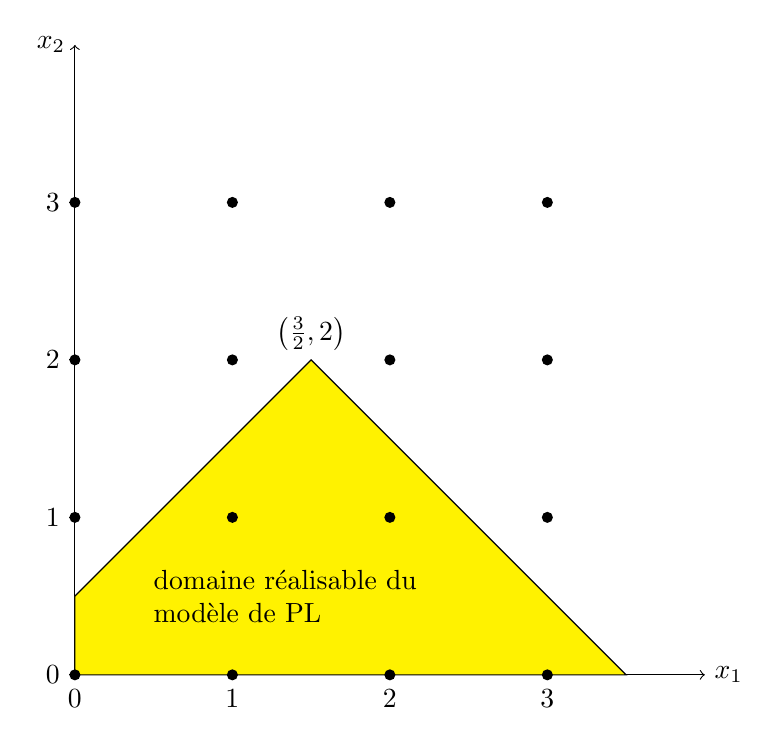
\begin{tikzpicture}[scale=2.00]
\draw[->] (0,0) -- (4,0) node[below,right] {$x_1$};
\draw[->] (0,0) -- (0,4) node[above,left] {$x_2$};

\foreach \x in {0,1,2,3}
  \draw (\x,1pt) -- (\x,-1pt) node[anchor=north] {$\x$};
\foreach \y in {0,1,2,3}
  \draw (1pt,\y) -- (-1pt,\y) node[anchor=east] {$\y$};

\filldraw[fill=yellow]
  (0,0) -- (0,0.5) -- (1.5,2) -- (3.5,0) -- (0,0);
  
\draw (1.5,0.5) node[text width=4cm,text ragged] {domaine réalisable du modèle de PL};

\draw (1.5,2) node[above]{$\left( \frac{3}{2},2\right)$};

\foreach \x in {0,1,2,3}
\foreach \y in {0,1,2,3}
\fill (\x,\y) circle (1 pt);;
\end{tikzpicture}
\caption{Exemple de relaxation linéaire: problème d'admissibilité des solutions}
\label{fig:relaxation_1}
\end{center}
\end{figure}
\end{example}

\begin{example}
Considérons le programme
\begin{align*}
\max\ & z = x_1+5x_2\\
\st & x_1+10x_2 \leq 20, \\
& x_2 \leq 2, \\
& x_1, x_2 \geq 0 \mbox{ et entiers}.
\end{align*}
La version relâchée de programme est
\begin{align*}
\max\ & z = x_1+5x_2\\
\st & x_1+10x_2 \leq 20, \\
& x_2 \leq 2, \\
& x_1, x_2 \geq 0,
\end{align*}
qui a pour solution optimale $(2,1.8)$. En arrondissant à $(2,1)$ afin de garantir l'admissibilité, nous obtenir la valeur 7 pour la fonction objectif, loin de la valeur optimale du programme mixte entier, avec pour valeur optimale 11, en $(0,2)$ (voir Figure~\ref{fig:relaxation_2}).
\begin{figure}[htb]
\begin{center}
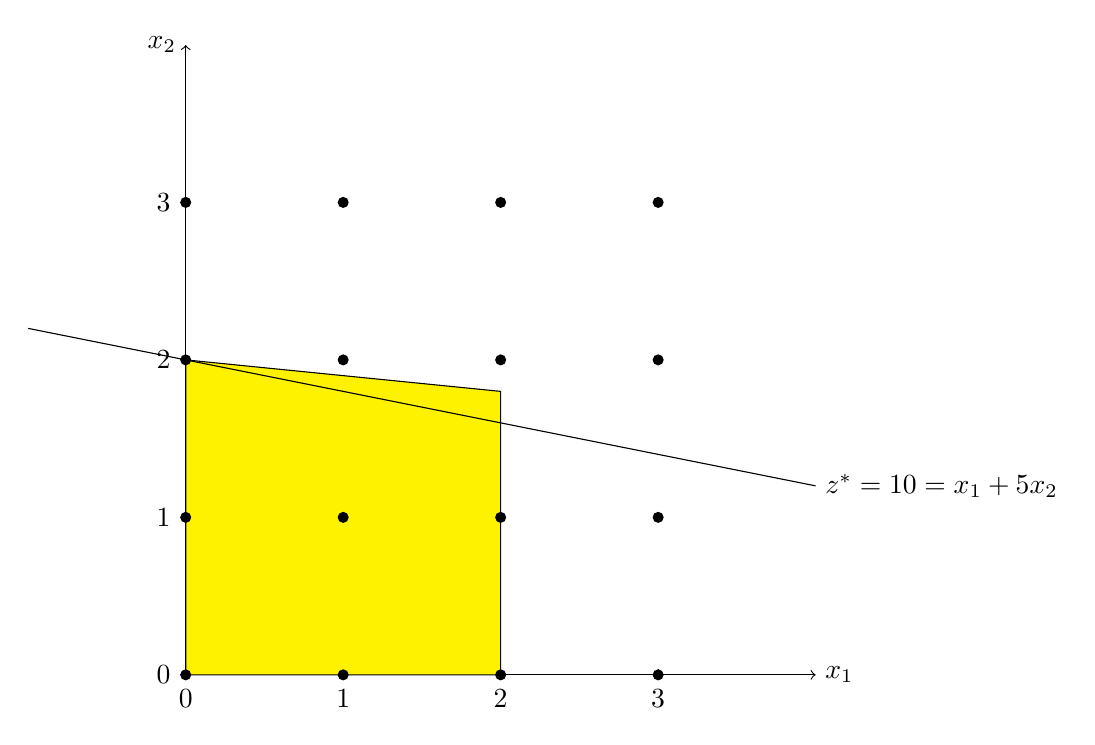
\begin{tikzpicture}[scale=2.00]
\draw[->] (0,0) -- (4,0) node[below,right] {$x_1$};
\draw[->] (0,0) -- (0,4) node[above,left] {$x_2$};

\foreach \x in {0,1,2,3}
  \draw (\x,1pt) -- (\x,-1pt) node[anchor=north] {$\x$};
\foreach \y in {0,1,2,3}
  \draw (1pt,\y) -- (-1pt,\y) node[anchor=east] {$\y$};

\filldraw[fill=yellow]
  (0,0) -- (0,2) -- (2,1.8) -- (2,0) -- (0,0);

\draw (-1,2.2) -- (4,1.2) node[above,right,sloped] {$z^* = 10 = x_1+5x_2$};

\foreach \x in {0,1,2,3}
\foreach \y in {0,1,2,3}
\fill (\x,\y) circle (1 pt);;
\end{tikzpicture}
\caption{Exemple de relaxation linéaire: solution médiocre}
\label{fig:relaxation_2}
\end{center}
\end{figure}
\end{example}

\subsection{Approche par énumération}

Un modèle en nombres entiers borné (par exemple, un modèle avec uniquement des variables 0--1) possède un nombre fini de solutions.
Nous pourrions envisagear de toutes les énumérer, mais le nombre de solutions explose rapidement. Pour $n = 20$ variables 0--1, il y a plus d'un million de solutions possibles.
Pour $n=30$, c'est plus d'un milliard.
Comme il apparaît qu'il est vite déraisonnable de procéder à une énumération complète des solutions, nous allons essayer de mettre à profit la relaxation en programme linéaire pour éliminer certaines de ces solutions.
Cette technique d'énumération partielle est connue sous le vocable de {\sl branch-and-bound} (B\&B).
Il s'agit d'une approche {\sl diviser-pour-régner}:
\begin{itemize}
\item
décomposition du problème en sous-problèmes plus simples;
\item
combinaison de la résolution de ces sous-problèmes pour obtenir la solution du problème original.
\end{itemize}
Dans l'algorithme de branch-and-bound, chaque sous-problème correspond à un sommet dans l'arbre des solutions.
Nous résolvons la relaxation linéaire de chaque sous-problème.
L'information tirée de la relaxation linéaire nous permettra (peut-être) d'éliminer toutes les solutions pouvant être obtenues à partir de ce sommet.

\subsubsection{Algorithme de branch \& bound: cas 0--1}

Un algorithme simple pour énumérer toutes les solutions d'un modèle 0--1 consiste à:
\begin{itemize}
\item
choisir un sommet dans l'arbre des solutions;
\item
choisir une variable $x$ non encore fixée relativement à ce sommet;
\item
générer les deux variables $x = 0$ et $x = 1$ (la variable $x$ est dite {\sl fixée}): chaque alternative correspond à un sommet de l'arbre des solutions;
\item
recommencer à partir d'un sommet pour lequel certaines variables ne sont pas encore fixées.
\end{itemize}
A la racine de l'arbre, aucune variable n'est encore fixée, tandis qu'aux feuilles de l'arbre, toutes les variables ont été fixées.
Le nombre de feuilles est $2^n$ (pour $n$ variables 0--1).

Le calcul de borne (ou évaluation) consiste à résoudre la relaxation linéaire en chaque sommet.
L'élagage (ou élimination) consiste à utiliser l'information tirée de la résolution de la relaxation linéaire pour éliminer toutes les solutions émanant du sommet courant.
Dés lors, le branch-and-bound est un algorithme de séparation et d'évaluation successives.

\begin{example}[California Mfg]
Rappelons le problème
\begin{align*}
max\ & z = 9x_1 + 5x_2 + 6x_3 + 4x_4 \\
\st & 6x_1 + 3x_2 + 5x_3 + 2x_4 \leq 10; \\
& x_3 + x_4 \leq 1; \\
& -x_1 + x_3 \leq 0; \\
& -x_2 + x_4 \leq 0; \\
& x_1, x_2, x_3, x_4 \leq 1; \\
& x_1, x_2, x_3, x_4 \geq 0; \\
& x_1, x_2, x_3, x_4 \mbox{ entiers}.
\end{align*}
La relaxation linéaire permet aux variables de prendre les valeurs fractionnaires entre 0 et 1, ce qui conduit à la solution
\[
\left( \frac{5}{6}, 1, 0, 1 \right),
\]
avec comme valeur $z = 16.5$.
Branchons sur la variable $x_1$.

Dénotons sous-problème 1 celui obtenu avec $x_1 = 0$:
\begin{align*}
max\ & z = 5x_2 + 6x_3 + 4x_4 \\
\st & 3x_2 + 5x_3 + 2x_4 \leq 10; \\
& x_3 + x_4 \leq 1; \\
& x_3 \leq 0; \\
& -x_2 + x_4 \leq 0; \\
& x_2, x_3, x_4 \mbox{ binaires}.
\end{align*}
La solution de la relaxation linéaire est $(x_1, x_2, x_3, x_4) = (0,1,0,1)$, avec $z = 9$.

Le sous-problème 2 est celui obtenu avec $x_1 = 1$:
\begin{align*}
max\ & z = 5x_2 + 6x_3 + 4x_4 + 9 \\
\st & 3x_2 + 5x_3 + 2x_4 \leq 4; \\
& x_3 + x_4 \leq 1; \\
& x_3 \leq 1; \\
& -x_2 + x_4 \leq 0; \\
& x_2, x_3, x_4 \mbox{ binaires}.
\end{align*}
La solution de la relaxation linéaire est alors
\[
(x_1, x_2, x_3, x_4) = \left( 1, \frac{4}{5},0, \frac{4}{5} \right),
\]
avec $z = 16+\frac{1}{5}$.
\end{example}

Nous obtenons dès lors les bornes suivantes:
\begin{itemize}
\item
sous-problème 1: $Z_1 \leq 9$;
\item
sous-problème 2: $Z_2 \leq 16+\frac{1}{5}$.
\end{itemize}
Notons que toutes les variables sont binaires et tous les paramètres dans l'objectif sont des valeurs entières.
Dès lors, la borne supérieure pour le sous-problème 2 est 16.
Pour le sous-problème 1, la solution obtenue est entiere: c'est la meilleure solution courante.
Nous savons que la valeur optimale cherchée, Z, sera au moins
\[
Z^* = 9: Z \geq Z^*.
\]

Quels sous-problèmes pouvons-nous à présent considérer afin de nous approcher de la solution optimale? Tous les sous-problèmes actuellement traités doivent-ils donner naissance à d'autres problèmes.
Si un sous-problème ne donne lieu à aucun autre problème, nous parlerons d'élagage, en référence avec l'idée de couper la branche correspondante dans l'arbre d'exploration.

Considérons tout d'abord le sous-probleme 1: la solution optimale de la relaxation PL est entière.
Il ne sert donc à rien de brancher sur les autres variables, puisque toutes les autres solutions entières (avec $x_1 = 0$) sont nécessairement de valeur inférieures ou égales à 9.
Nous pouvons donc élaguer ce sommet.

Pour le sous-probleme 2, la solution optimale de la relaxation PL n'est pas entière:
\[
Z^* = 9 \leq Z \leq 16.
\]
La branche ($x_1 = 1$) peut encore contenir une solution optimale.
Mais si nous avions eu $Z_2 \leq Z*$, nous aurions pu conclure que la
branche ne pouvait améliorer la meilleure solution courante.

Un sous-problème est elagué si une des trois conditions suivantes est satisfaite :
\begin{itemize}
\item
test 1: sa borne supérieure (valeur optimale de la relaxation PL) est inférieure ou égale à $Z^*$ (valeur de la meilleure solution courante);
\item
test 2: sa relaxation PL n'a pas de solution réalisable;
\item
test 3: la solution optimale de sa relaxation PL est entière.
\end{itemize}
Lorsque le test 3 est verifié, nous testons si la valeur optimale de la relaxation PL du sous-problème, $Z_i$, est supérieure à $Z^*$.
Si $Z_i > Z^*$, alors $Z^* := Z_i$, et nous conservons la solution, qui
devient la meilleure solution courante.
En résumé, nous obtenons l'algorithme ci-dessous.
\begin{algo}{Branch-and-Bound: cas binaire}
\begin{enumerate}
\item
Initialisation:
\begin{enumerate}[(a)]
\item
poser $Z^* = -\infty$;
\item
appliquer le calcul de borne et les critères d'élagage à la racine (aucune variable fixée).
\end{enumerate}
\item
Critere d'arrêt : s'il n'y a plus de sous-problemes non élagués, arrêter.
\item
Branchement:
\begin{enumerate}[(a)]
\item
parmi les sous-problèmes non encore élagués, choisir celui qui a été crée le plus récemment (s'il y a égalité, choisir celui de plus grande borne supérieure);
\item
appliquer le Test 1: si le sous-problème est élagué,
retourner en 2.
\item
brancher sur la prochaine variable non fixée.
\end{enumerate}
\item
Calcul de borne:
\begin{enumerate}[(a)]
\item
résoudre la relaxation PL de chaque sous-problème;
\item
arrondir la valeur optimale si tous les paramètres de l'objectif sont entiers.
\end{enumerate}
\item
Elagage: élaguer un sous-problème si
\begin{enumerate}[(a)]
\item
la borne superieure est inférieure ou égale à $Z^*$;
\item
la relaxation PL n'a pas de solution réalisable;
\item
la solution optimale de la relaxation PL est entière: si la borne supérieure est strictement supérieure à $Z^*$, $Z^*$ est mise à jour et la solution de la relaxation PL devient la meilleure solution courante.
\end{enumerate}
\item
 Retourner en 2.
\end{enumerate}
\end{algo}

A partir de quel noeud devrions-nous brancher? Il y a plusieurs choix possibles; dans cette version, on propose comme règle de sélection de choisir le sous-problème le plus récemment créé.
L'avantage est que cette approche facilite la réoptimisation lors du calcul de borne, car il n'y a que peu de changements apportés par rapport au dernier sous-probleme traité.
Le désavantage est que cela peut créer un grand nombre de sous-probèmes.
Une autre option est la règle de la meilleure borne: choisir le sous-problème ayant la plus grande borne supérieure.

Dans cette version, la règle de branchement consiste à choisir la prochaine variable non fixée. Il est souvent plus intéressant de choisir une variable à valeur fractionnaire.
En branchant sur une telle variable, il est certain que les deux sous-problèmes crées mènent à des solutions differentes de la solution courante.
De nombreux critères existent pour choisir une telle variable de facon à orienter la recherche vers un élagage rapide.

\begin{example}[suite]
Jusqu'à maintenant, voici l'arbre obtenu, en branchant sur la variable $x_1$.
\begin{center}
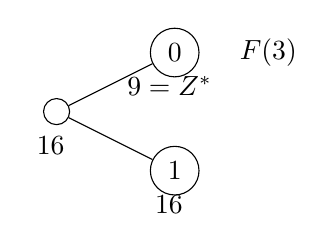
\begin{tikzpicture}
\node (root) [circle,draw] {} [grow'=right]
child {node (A) [circle,draw] {0}}
child {node (B) [circle,draw] {1}};
\draw (root) node[below, text width=5mm, text ragged]{\hspace{5mm} 16}; 
\draw (B) node[below, text width=5mm, text ragged]{\hspace{5mm} 16}; 
\draw (A) node[below, text width=12mm, text ragged]{\hspace{12mm} $9 = Z^*$}; 
\draw (A) node[right] {\qquad $F(3)$};
 \end{tikzpicture}
\end{center}
$F(3)$ indique que le sous-probleme a été élagué ({\sl fathomed}) en raison du Test 3.

Sélection: nous choisissons le sous-problème 2, le seul qui n'a pas encore été élagué.
Nous branchons sur la prochaine variable, soit $x_2$.
Deux nouveaux sous-problèmes sont crées:
\begin{itemize}
\item
sous-problème 3: $x_1 = 1$, $x_2 = 0$;
\item
sous-problème 4: $x_1 = 1$, $x_2 = 1$.
\end{itemize}

Considérons tout d'abord le sous-problème 3 ($x_1 = 1$, $x_2 = 0$).
Nous obtenons le problème
\begin{align*}
\max z_3 =\ & 6x_3 + 4x_4 + 9 \\
\st{} & 5 x_3 + 2x_4 \leq 4 \\
& x_3 + x_4 \leq 1 \\
& x_3 \leq 1 \\
& x_4 \leq 0 \\
& x_3,\ x_4 \mbox{ binaire}.
\end{align*}
La solution de la relaxation PL est
\[
( x_1, x_2, x_3, x_4) = \left(1,0, \frac{4}{5},0 \right).
\]
 et
 \[
Z = 13+\frac{4}{5}:\ Z_3 \leq 13.
 \]
 
Le sous-problème 4 ($x_1 = 1$, $x_2 = 1$) devient
\begin{align*}
\max z_4 =\ & 6x_3 + 4x_4 + 14 \\
\st{} & 5 x_3 + 2x_4 \leq 1 \\
& x_3 + x_4 \leq 1 \\
& x_3 \leq 1 \\
& x_4 \leq 1 \\
& x_3,\ x_4 \mbox{ binaire}.
\end{align*}
La solution de la relaxation PL est
\[
( x_1, x_2, x_3, x_4) = \left(1,1,0, \frac{1}{2} \right).
\]
 et
 \[
Z = 16:\ Z_4 \leq 16.
 \]

Aucun des tests d'élagage ne s'applique sur ces sous-problèmes.
Nous devons dès lors choisir un des deux sous-problèmes pour effectuer un branchement, puisque ce sont ceux crées le plus récemment.
Nous choisissons celui de plus grande borne supérieure, soit le sous-problème 4.
Nous branchons sur $x_3$ et nous générons deux nouveaux sous-problèmes.

Le sous-problème 5, défini avec $x_1 = 1$, $x_2 = 1$, $x_3 = 0$, s'écrit
\begin{align*}
\max z_5 =\ & 4x_4 + 14 \\
\st{} & 2x_4 \leq 1 \\
& x_4 \leq 1 \\
& x_4 \leq 1 \\
& x_4 \mbox{ binaire}.
\end{align*}
La solution de la relaxation PL est
\[
( x_1, x_2, x_3, x_4) = \left(1,1,0, \frac{1}{2} \right)
\]
et
\[
Z = 16:\ Z_5 \leq 16.
\]

Le sous-problème 6, défini avec $x_1 = 1$, $x_2 = 1$, $x_3 = 1$, s'écrit
\begin{align*}
\max z_5 =\ & 4x_4 + 20 \\
\st{} & 2x_4 \leq -4 \\
& x_4 \leq 0 \\
& x_4 \leq 1 \\
& x_4 \mbox{ binaire}.
\end{align*}
La relaxation PL n'a pas de solution realisable: ce sous-probleme est élagué.

Le sous-problème 5 ne peut pas être élagué.
Il est crée le plus récemment parmi les sous-problèmes non élagués (3 et 5), aussi choisissons-nous le pour effectuer un branchement.
Nous branchons sur $x_4$ et générons les sous-problèmes suivants:
\begin{itemize}
\item
sous-problème 7: $x_1 = 1$, $x_2 = 1$, $x_3 = 0$, $x_4 = 0$;
\item
sous-problème 8: $x_1 = 1$, $x_2 = 1$, $x_3 = 0$, $x_4 = 1$.
\end{itemize}
Toutes les variables sont fixées, aussi pouvons-nous directement résoudre ces sous-problèmes. 
Le sous-problème 7 a pour solution $(x_1, x_2, x_3, x_4) = (1, 1, 0, 0)$, pour $Z_7 = 14$.
La solution est entière, aussi nous élaguons le sous-problème en vertu du Test 3.
Puisque $Z_7 > Z^*$, $Z^* = 14$ et la solution du sous-problème devient la meilleure solution courante.
Le sous-problème 8 a pour solution $(x_1, x_2, x_3, x_4) = (1, 1, 0, 1)$.
Cette solution n'est pas réalisable, car la première contrainte $(2x_4 \leq 1)$ est violée.
Le sous-problème est par conséquent élagué par le Test 2.

Le sous-problème 3 est le seul non encore élagué.
Appliquons le Test 1: $Z_3 = 13 \leq 14 = Z*$.
Le sous-problème est donc elagué.
Comme il n'y a plus de sous-problèmes non élagués, nous pouvons nous arrêter.
La solution optimale est:
\[
(x_1, x_2, x_3, x_4) = (1,1,0,0),
\]
et la valeur optimale est $Z^* = 14$.

L'arbre obtenu suite à l'exécution de l'algorithme se présente comme suit:
\begin{center}
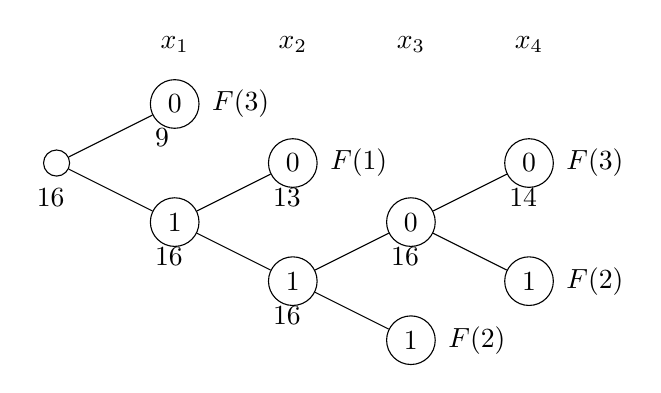
\begin{tikzpicture}
\node (root) [circle,draw] {} [grow'=right]
child {node (A) [circle,draw] {0}}
child {node (B) [circle,draw] {1}
  child {node (C) [circle,draw] {0}}
  child {node (D) [circle,draw] {1}
    child {node (E) [circle,draw] {0}
      child {node (F) [circle,draw] {0}}
      child {node (G) [circle,draw] {1}}
    }
    child {node (H) [circle,draw] {1}}
  }
 };
\draw (root) node[below, text width=5mm, text ragged]{\hspace{5mm} 16}; 
\draw (B) node[below, text width=5mm, text ragged]{\hspace{5mm} 16}; 
\draw (A) node[below, text width=5mm, text ragged]{\hspace{5mm} 9}; 
\draw (D) node[below, text width=5mm, text ragged]{\hspace{5mm} 16}; 
\draw (C) node[below, text width=5mm, text ragged]{\hspace{5mm} 13}; 
\draw (E) node[below, text width=5mm, text ragged]{\hspace{5mm} 16}; 
\draw (F) node[below, text width=5mm, text ragged]{\hspace{5mm} 14}; 
\draw (A) node[right] {\quad $F(3)$};
\draw (F) node[right] {\quad $F(3)$};
\draw (C) node[right] {\quad $F(1)$};
\draw (G) node[right] {\quad $F(2)$};
\draw (H) node[right] {\quad $F(2)$};
\draw (1.5,1.5) node {$x_1$};
\draw (3,1.5) node {$x_2$};
\draw (4.5,1.5) node {$x_3$};
\draw (6,1.5) node {$x_4$};
 \end{tikzpicture}
\end{center}
$F(j)$: le sous-problème est élagué par le Test j
\end{example}

\subsubsection{Algorithme de branch \& bound: cas général}

Considérons à présent le cas général d'un modèle de programmation (mixte) en nombres entiers: variables entières générales et variables continues.
Comme précédemment, nous ignorons dans un premier temps les contraintes d'intégralité (les valeurs des variables entières sont traitées comme variables continues), et résolvons le programme linéaire résultant.
Si la solution optimale de ce programme satisfait aux contraintes d'intégralité, alors cette solution est aussi solution optimale du programme avec variables entières.
Sinon, il doit exister au moins une variable $x_j$ dont la valeur $\alpha$ est fractionnaire.
La procédure de branchement se généralise alors comme suit: nous séparons alors le problème relaxé en deux sous-problèmes;
un sous-problème contiendra la contrainte $x_j \leq \lfloor \alpha \rfloor$ et le second la contrainte $x_j \geq \lceil \alpha \rceil  = \lfloor \alpha \rfloor + 1$.
Nous répétons le processus pour chacun des sous-problèmes.
Cette procédure est habituellement représentée sous forme
d'un arbre binaire où, à chaque niveau, une partition du sommet père s'effectue suivant la règle décrite précédemment.
Il s'agit alors de parcourir cet arbre d'énumération afin d'y trouver la solution optimale.
L'exploration d'un chemin de l'arbre peut prendre fin pour trois raisons:
\begin{itemize}
\item
la solution devient entière;
\item
le domaine admissible d'un sous-problème devient vide;
\item
la valeur de l'objectif correspondant à la solution optimale du problème relaxé est inférieure (moins bonne) à celle d'une solution admissible connue, possiblement obtenue à un autre sommet de l'arbre.
\end{itemize}
Dans chacun de ces trois cas on dit que le sommet est sondé, et il est inutile de pousser plus loin dans cette direction.
L'algorithme s'arrête lorsque tous les sommets sont sondés.
La meilleure solution obtenue au cours du déroulement de l'algorithme est alors l'optimum global de notre problème.

\begin{algo}{Algorithme de B\&B: cas général}
\begin{enumerate}
\item
Initialisation:
\begin{enumerate}[(a)]
\item
 Poser $Z^* = -\infty$.
\item
 Appliquer le calcul de borne et les critères d'élagage à la racine (aucune variable fixée).
\item
 Critere d'arrêt : s'il n'y a plus de sous-problèmes non élagués, arrêter.
 \end{enumerate}
\item
 Branchement:
 \begin{enumerate}[(a)]
 \item
  Parmi les sous-problèmes non encore élagués, choisir celui qui a été crée le plus récemment (s'il y a égalité, choisir celui de plus grande borne supérieure).
 \item
  Appliquer le Test 1: si le sous-problème est élagué, retourner en 2.
 \item
  Brancher sur la prochaine variable entière à valeur non entière dans la relaxation PL.
 \end{enumerate}
\item
 Calcul de borne: résoudre la relaxation PL de chaque sous-problème.
\item
  Elagage: élaguer un sous-problème si
  \begin{enumerate}[(a)]
  \item
   La borne superieure est inférieure ou égale à $Z^*$.
  \item
   La relaxation PL n'a pas de solution réalisable.
  \item
   Dans la solution optimale de la relaxation PL, toutes les variables entières sont à valeurs entières: si la borne
supérieure est strictement supérieure à $Z^*$, $Z^*$ est mise à jour et la solution de la relaxation PL devient la meilleure solution courante.
 \end{enumerate}
\item
 Retourner en 2.
\end{enumerate}
\end{algo}

\subsection{Les hyperplans coupants (méthode de coupe)}

Vu que l'énumération des variables entières peut être coûteuse, l'idée est d'ajouter des contraintes redondantes pour le modèle en nombres entiers, mais non pour la relaxation PL.

\begin{example}
Considérons le programme mathématique
\begin{align*}
\max_x \ & 4x_1 + \frac{5}{2} x_2 \\
& x_1 + x_2 \leq 6 \\
& 9x_1 + 5x_2 \leq 45 \\
& x_1,\ x_2 \in \NN.
\end{align*}
Le dictionnaire optimal correspondant à la relaxation linéaire de ce programme contient les deux contraintes
\begin{align*}
x_1 & = \frac{15}{4} + \frac{5}{4}x_3 - \frac{1}{4}x_4, \\
x_2 & = \frac{9}{4} - \frac{9}{4}x_3 + \frac{1}{4}x_4, \\
\end{align*}
où $x_3$ et $x_4$ sont des variables d'écart.
Puisque la variable de base $x_1$ n'est pas entière, cette solution de
base n'est pas admissible.
nous pouvons réécrire la première contrainte sous la forme
\begin{align*}
x_1 - \frac{5}{4}x_3 + \frac{1}{4}x_4 = \frac{15}{4}.
\end{align*}
En utilisant l'identité
\[
a = \lfloor a \rfloor + (a - \lfloor a \rfloor),
\]
où $(a - \lfloor a \rfloor)$ représente la partie fractionnaire de $a$ $(0 \leq a - \lfloor a \rfloor < 1)$, nous obtenons
\[
x_1 + \left(
\left\lfloor -\frac{5}{4} \right\rfloor + \frac{3}{4} \right)x3 + 
\left(\left\lfloor\frac{1}{4}\right\rfloor + \frac{1}{4} \right) x_4 =
\left(\left\lfloor \frac{15}{4} \right\rfloor + \frac{3}{4} \right),
\]
c'est-à-dire, en mettant tous les coefficients entiers à gauche et les coefficients fractionnaires à droite:
\[
x_1 - 2x_3 - 3 = \frac{3}{4} - \frac{3}{4}x_3 - \frac{1}{4}x_4.
\]
Puisque les variables $x_3$ et $x_4$ sont non négatives, la partie fractionnaire (constante du membre de droite) est inférieure à 1, le membre de droite est strictement inférieur à 1. Puisque le membre de gauche est entier, le membre de droite doit aussi être entier.
Or un entier inférieur à 1 doit être inférieur ou égal à zéro.
Nous en déduisons une contrainte additionnelle qui doit être satisfaite par toute solution admissible du problème originel, et que ne satisfait pas la solution de base courante:
\begin{align*}
\frac{3}{4}-\frac{3}{4}x_3 - \frac{1}{4}x_4 \leq 0.
\end{align*}
En utilisant les identités $x_3 = 6 - x_1 - x_2$ et $x_4 = 45 - 9x_1 - 5x_2$, nous obtenons la coupe sous sa forme géométrique:
\[
3x_1 + 2x_2 \leq 15.
\]
Cette contrainte linéaire rend inadmissible la solution courante admissible, sans éliminer aucune autre solution entière. Si la solution du nouveau problème est entière, il s'agit de la solution optimale de notre problème.
Sinon, nous construisons une nouvelle coupe et recommençons.
%La résolution du nouveau programme linéaire s'effectue, comme dans l'algorithme de branch-
%and-bound, à l'aide de l'algorithme du simplexe appliqué au problème dual, afin de tirer profit de la solution duale optimale obtenue précédemment. Cette partie doit être mieux justifiée, en se basant sur le fait que le dual reste réalisable.
\end{example}

\begin{example}
Reprenons le problème, illustré sur la Figure~\ref{fig:cutting},
\begin{align*}
\max\ & z = 3x_1 + 2x_2 \\
\st & 2x_1 + 3x_2 \leq 4, \\
& x_1, x_2 \mbox{ binaire}.
\end{align*}
Les solutions réalisables sont $(0,0)$, $(1,0)$ et $(0,1)$.
\begin{figure}[htbp]
\begin{center}
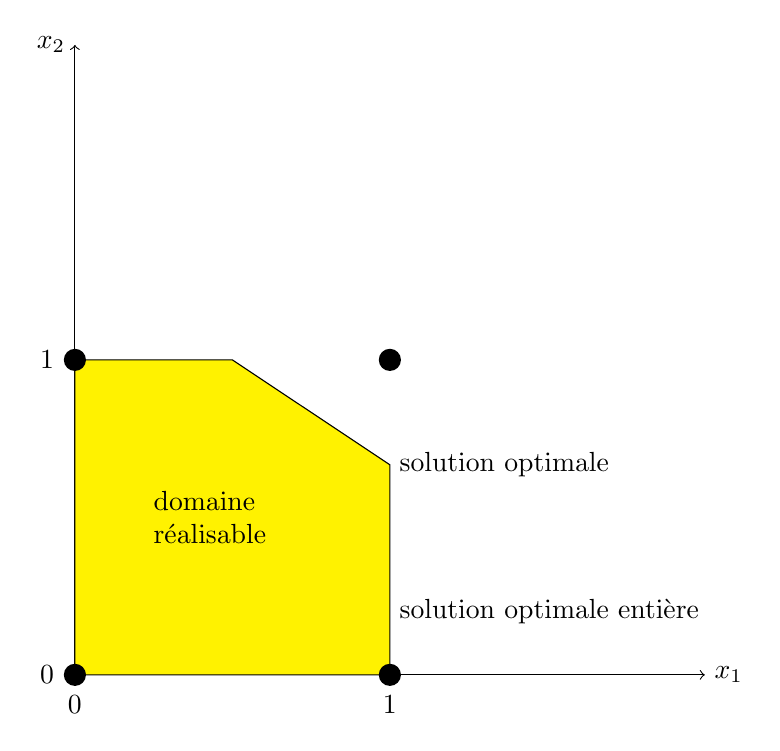
\begin{tikzpicture}[scale=4]
\draw[->] (0,0) -- (2,0) node[below,right] {$x_1$};
\draw[->] (0,0) -- (0,2) node[above,left] {$x_2$};

\foreach \x in {0,1}
  \draw (\x,1pt) -- (\x,-1pt) node[anchor=north] {$\x$};
\foreach \y in {0,1}
  \draw (1pt,\y) -- (-1pt,\y) node[anchor=east] {$\y$};

\filldraw[fill=yellow]
  (0,0) -- (0,1) -- (0.5,1) -- (1,0.667) -- (1,0) -- (0,0);
  
\draw (0.5,0.5) node[text width=2cm,text ragged] {domaine réalisable};

\foreach \x in {0,1}
\foreach \y in {0,1}
\fill (\x,\y) circle (1 pt);;

\draw (1,0.667) node[above,right] {solution optimale};
\draw (1,0.2) node[above,right] {solution optimale entière};

\end{tikzpicture}
\end{center}
\caption{Méthode de coupes}
\label{fig:cutting}
\end{figure}

Une contrainte redondante est:
\[
x_1 + x_2 \leq 1.
\]
Suite à l'ajout de la contrainte redondante, comme représenté sur la Figure~\ref{fig:cutting_2}, le problème est résolu à la racine.
\begin{figure}[htb]
\begin{center}
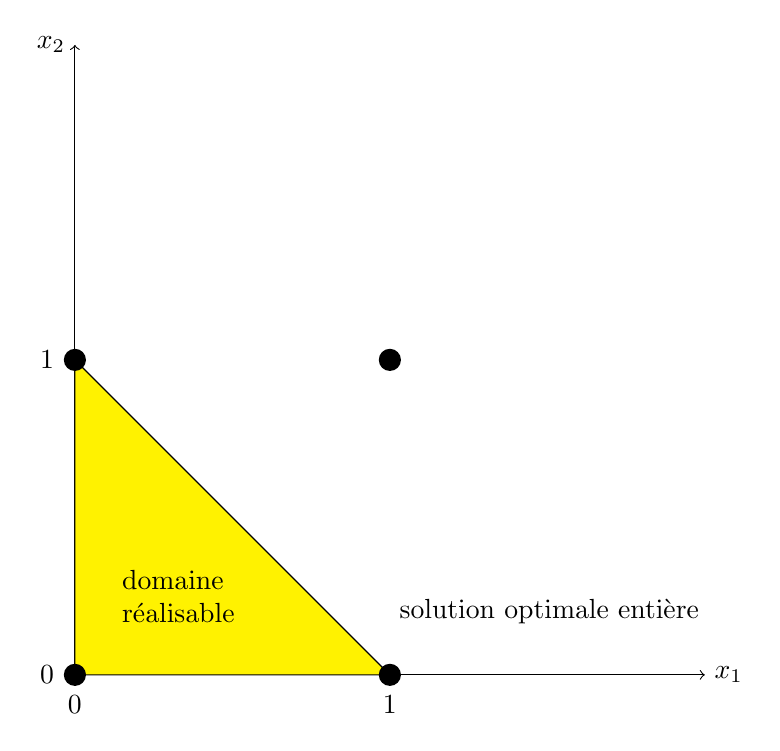
\begin{tikzpicture}[scale=4]
\draw[->] (0,0) -- (2,0) node[below,right] {$x_1$};
\draw[->] (0,0) -- (0,2) node[above,left] {$x_2$};

\foreach \x in {0,1}
  \draw (\x,1pt) -- (\x,-1pt) node[anchor=north] {$\x$};
\foreach \y in {0,1}
  \draw (1pt,\y) -- (-1pt,\y) node[anchor=east] {$\y$};

\filldraw[fill=yellow]
  (0,0) -- (0,1) -- (1,0) -- (0,0);
  
\draw (0.4,0.25) node[text width=2cm,text ragged] {domaine réalisable};

\foreach \x in {0,1}
\foreach \y in {0,1}
\fill (\x,\y) circle (1 pt);;

\draw (1,0.2) node[above,right] {solution optimale entière};

\end{tikzpicture}
\end{center}
\caption{Méthode de coupes: ajout d'une contrainte}
\label{fig:cutting_2}
\end{figure}
\end{example}

Il y a plusieurs algorithmes permettant de générer de telles inégalités redondantes, appelées coupes.
Mais il est rare que leur ajout permette de résoudre le probleme à la racine.
L'ajout de coupes permet toutefois de réduire le nombre de sous-problèmes traités par l'algorithme de Branch-and-Bound.
Nous pouvons même ajouter des coupes pour chaque sous-problème (pas seulement à la racine): nous obtenons alors un algorithme de branch-and-cut.

\section{Modélisation avec GAMS}

\begin{example}[Echangeurs de chaleur]
Considérons un problème simplifié d'affection de flux de processus à des échangeurs de chaleur;
les échangeurs de chaleur ont pour but de transférer la chaleur d'un flux chaud à un flux froid, afin de limiter la consommation d'énergie nécessaire pour chauffer ou refroidir des flux liquides (par exemple de l'eau) intervenant dans des processus de production industrielle.
Le problème d'optimisation correspondant est:
\begin{align*}
\min\ z &= \sum_{i = 1}^n \sum_{j =1}^n c_{ij}x_{ij} \\
\sc{} & \sum_{i = 1}^n x_{ij} = 1,\ j= 1,\ldots,n, \\  
& \sum_{j = 1}^n x_{ij} = 1,\ i=1,\ldots,n, \\ 
& x_{ij} \in \lbrace 0, 1 \rbrace,\ i=1,\ldots,n,\ j=1,\ldots,n, 
\end{align*}
ce qui n'est rien d'autre qu'un problème classique d'affection.
$i$ représente ici l'indice des $n$ flux, et $j$, l'indice des $n$ échangeurs.
La variable binaire $x_{ij}$ vaut 1 si le flux $i$ est affecté à l'échangeur $j$, et 0 sinon.
Les contraintes indiquent que chaque échangeur doit être affecté à un flux, et réciproquement.
Les coûts $c_{ij}$ d'affectation des flux aux échangeur sont résumés dans la Table~\ref{tab:streams}. 
\begin{figure}[htb]
\begin{center}
\begin{tabular}[b]{|c|c|c|c|c|}
\hline
\backslashbox{Echangeur}{Flux} & 1 & 2 & 3 & 4 \\
\hline
A & 94 & 1 & 54 & 68 \\
\hline
B & 74 & 10 & 88 & 82 \\
\hline
C & 73 & 88 & 8 & 76 \\
\hline
D & 11 & 74 & 81 & 21 \\
\hline
\end{tabular}
\end{center}
\caption{coûts d'affectation des échangeurs de chaleur}
\label{tab:streams}
\end{figure}
Le problème peut se formuler en GAMS comme
\begin{verbatim}
HEAT.GMS 

$TITLE Test Problem 
$OFFSYMXREF 
$OFFSYMLIST 

SETS 
     I  streams     / A, B, C, D / 
     J  exchangers  / 1*4 / ; 

 TABLE C(I,J) Cost of assigning stream i to exchanger j 

         1    2    3    4 
    A   94    1   54   68 
    B   74   10   88   82 
    C   73   88    8   76 
    D   11   74   81   21 ; 
 

 VARIABLES X(I,J), Z; 
 BINARY VARIABLES X(I,J); 

 EQUATIONS ASSI(J), ASSJ(I), OBJ; 

 ASSI(J).. SUM( I, X(I,J) ) =E= 1; 
 ASSJ(I).. SUM( J, X(I,J) ) =E= 1; 
 OBJ..     Z =E= SUM ( (I,J), C(I,J)*X(I,J) ) ; 

 MODEL HEAT / ALL /; 

 OPTION LIMROW = 0; 
 OPTION LIMCOL = 0; 
 OPTION SOLPRINT = OFF; 

 SOLVE HEAT USING MIP MINIMIZING Z; 

 DISPLAY X.L, Z.L ;  
 \end{verbatim}
La commende \verb|OPTION SOLPRINT=OFF| supprime l'impression de la solution; la sortie sera contrôlée par la commande \verb|DISPLAY| placé juste à
 la suite.
\end{example}

\begin{example}[Problème de production]
Nous souhaitons maximiser le profit que nous pourrions obtenir en considérant 3 produits.
Il n'y a pas coût de productions unitaires, mais des coûts fixes sont présent pour le premier et le deuxième produits.
Chaque produit est stocké, et nous ne pouvons pas dépasser le volume disponible.
Le code GAMS du problème est
\begin{verbatim}
 VARIABLES
  z                    profit;

POSITIVE VARIABLES
  x1                   produit1
  x2                   produit2
  x3                   produit3;

BINARY VARIABLES
  y1
  y2                           ;

EQUATIONS
  Objective             Maximize profit
  Ressource
  Upper1                limit on product 1
  Upper2                limit on product 2
  Upper3                limit on product 3;

Objective..
  z =E= 2*x1 + 3*x2 + 0.8*x3 - 3*y1 - 2*y2;

Ressource..
  0.2*x1 + 0.4*x2 + 0.2*x3 =L= 1;

Upper1..
  x1 =L= 3*y1;

Upper2..
  x2 =L= 2*y2;
1
Upper3..
  x3 =L= 5;

MODEL example /ALL/;

OPTION optcr = 0.05;

SOLVE example USING mip maximizing z;
\end{verbatim}
Notons la ligne
 \begin{verbatim}
OPTION optcr = 0.05;
\end{verbatim}
qui nous donne le critère d'optimalité sur la valeur optimale.
Dans le cas présent, nous exigeons que l'écart relatif entre la borne supérieur et la borne inférieure soit inférieur à 5\%.
\end{example}

\section{Exercices}

\begin{exercise}[Hillier et Lieberman~\cite{HillLieb01}, Exercice 12.7-9]
Utiliser l'algorithme de Branch \& Bound pour résoudre le problème
\begin{align*}
\max z\ &= 3x_1 + 4x_2 + 2x_3 + x_4 +2x_5,\\
\st{}\ & 2x_1 - x_2 + x_3 + x_4 +x_5 \leq 3, \\
& -x_1+3x_2 + x_3 - x_4 - 2x_5 \leq 2, \\
& 2x_1 + x_2 - x_3 + x_4 +3x_5 \leq 1,\\
& x_j \geq 0,\ j = 1,2,3,4,5,\\
& x_j \in \lbrace 0, 1\rbrace,\ j = 1, 2, 3.
\end{align*}
\end{exercise}

\section{Notes}

Le contenu de ce chapitre est repris des notes de cours de Patrice Marcotte (2001) et de Bernard Gendron (2007).
L'exemple GAMS sur les échangeurs de chaleur est dû à Grossmann.